% Chapter Template

\chapter{Solution Design} % Main chapter title

\label{Chapter4} % Change X to a consecutive number; for referencing this chapter elsewhere, use \ref{ChapterX}

\section{General Approach} \label{sec:generalApproach}

With the aim of complete the objectives mentioned in Sec.\ref{sec:thesisGoals}, a workflow was designed. This work flow contains five stages.

\begin{enumerate}
	\item Instrumentation of the applications
	\item Exploration
	\item Coverage measurement
	\item Summarize data
	\item Data Analysis
\end{enumerate}

\begin{figure}[h]
\centering
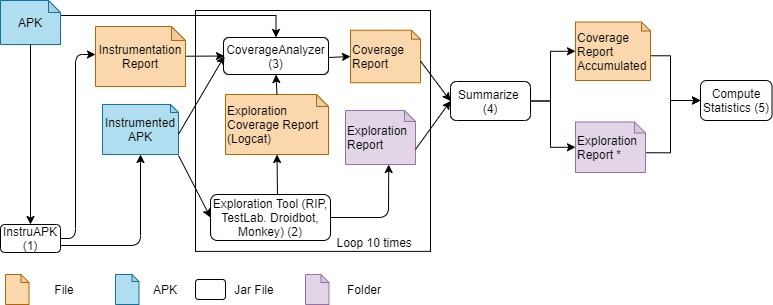
\includegraphics[width=0.8\textwidth]{../Figures/workflow.jpg}
\label{fig:workflow}
\caption{Main Workflow}
\end{figure}

%TODO agregar más explicación del workflow, como qué es la entrada y qué es la salida de cada punto, tal vez explicar un poco qué hace la etapa más no la herramienta o lo demás, explicar tal vez por qué es necesario y en qué ayuda cada etapa.


For the first stage, InstruAPK was used to make the instrumentation of the applications. This tool only takes into account the methods under the package name of the application that is being analysed. As a result, methods from different libraries are not being taken into count. The input for this stage is the original APK file, and the output is the instrumented APK together with the instrumentation report containing general information such as the file path, method's name, file name, and the method arguments, as well as a sequential number that will help us to know the total amount of instrumented methods and will work as their unique identifier.

The exploration was made by four different exploration tools, i. Droidbot, ii. Monkey, iii. Firebase Test Lab, and iv. RIP. Every tool was run to explore with a maximum time of 30 minutes. It is important to notice that, even when the max execution time seems to be short, it was enough for most of the application. This was because of the size of the applications, if the application is small, then the coverage will increase rapidly, because a bug was found during the exploration, or even because the tool marks the exploration as done. 

This stage input is only the instrumented APK file, and its output is the exploration report that every tool provides. I took the logcat from the exploration report, but when it was not available in it, which was the case of Monkey, it was extracted by using the adb shell command. The other three tools got the information at the end of their exploration.
 
%TODO poner la referencia del comando adb shell para el logcat https://developer.android.com/studio/command-line/logcat

Some of these tools, Droidbot, Monkey and Test Lab, were selected because of their high use in the industry and the remaining one was selected because of personal interest owing to it is an active project at the University of Los Andes inside the research group The Software Design Lab were I make part of. 

In stage 3, \textbf{CoverageAnalyzer (CA)} was used to make the coverage measurement and search for error lines. This stage inputs are the original APK, the instrumentation report and the instrumented APK, both from stage 1, and the logcat from stage 2. Its output is a report containing two method coverage measurements, the first one, calculated using the number of methods reported by APKAnalyzer, a tool provided for Google, and the second one with the number of instrumented methods reported by InstruAPK.

%TODO poner referencia de APKAnalyzer https://developer.android.com/studio/command-line/apkanalyzer

Stages 2. and 3. were repeated 10 times for every application that was selected, that leaded to the stage 4. The multiple executions are intending to get average values as well as comparable results along the different exploration tools. The input for this stage are all the method coverage reports from of the stage 3 as well as the exploration report from stage 2. The output are the accumulated method coverage by each tool for each application, which was calculated taking the unique methods called over all the ten executions, the average accumulated method coverage over time, as well as the number of errors and its average found per application.

The final stage encompasses data understanding, graphs creation, comparison using the graph and analysis of different qualitative aspects of every exploration tool. Thus, 

Any person can reproduce this work flow who desires to compare different exploration tools, even can make use of the same tools for the instrumentation and the coverage measurement, allowing easy and fast comparisons. Consequently, the decision-making starts to be easier for developers and researchers. Also,gives the possibility to researchers of compare their own exploration tools in a effortless and quick way.


%TODO citate InstruAPK repository
%TODO citate CA repository

\section{InstruAPK}\label{sec:instruAPK}

This tool was developed mainly for this study. It uses APKTool, a known Java application that allows inverse engineering in Android apps, allowing applications' instrumentation without the need of recompiling their source code. APKTool decodes the apk and the result is the smali representation of the app source code, These smali files are analysed in order to find all the methods to be instrumented and then, the log code is injected at the very beginning of each method. It is important to notice that no external libraries methods are instrumented. InstruAPK only search for methods following the android project structure that uses the application package name to store the application source code.

\begin{figure}[h]
\centering
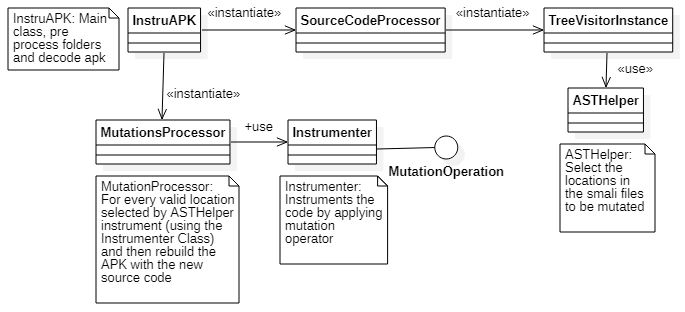
\includegraphics[width=0.8\textwidth]{../Figures/ClassDiagramInstruAPK.jpg}
\label{fig:instruAPK}
\caption{Class Diagram InstruAPK}
\end{figure}


%TODO explain the architecture and the tool in more detail, do not throw the image and just that.
\section{Coverage Analyser (CA)}\label{sec:ca}

This tool is also a Java Application created mainly for this study. It extracts all data from the log lines injected by InstruAPK and also the errors found under the application package name. When an instrumented application is ran, the logcat will contain the log lines with all the data. The logcat is stored in a txt file and that is what CA uses as its input filtering the results using the package name of the application being analysed. For the coverage measurement the tool uses the number of instrumented methods included in the InstruAPK instrumentation report As it was mentioned before, CA depends totally on the information provided by InstruAPK, CA can be seen as a complement of it, rather than an separate application.

\begin{figure}[h]
\centering
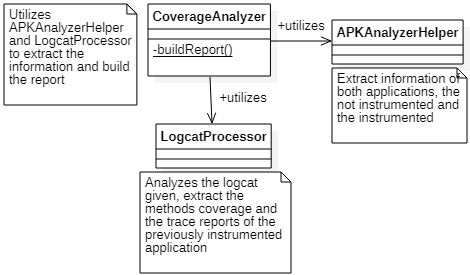
\includegraphics[width=0.8\textwidth]{../Figures/ClassDiagramCA.jpg}
\label{fig:ca}
\caption{Class Diagram Coverage Analyser}
\end{figure}

%TODO explain the architecture and the tool in more detail, do not throw the image and just that.